\documentclass{beamer}
\usepackage{listings}
\lstset{
%language=C,
frame=single, 
breaklines=true,
columns=fullflexible
}
\usepackage{blkarray}
\usepackage{subcaption}
\usepackage{url}
\usepackage{tikz}
\usepackage{subfig}
\usepackage{subcaption}
\usepackage{caption}
\usepackage[demo]{graphicx}
\usepackage{tkz-euclide} % loads  TikZ and tkz-base
%\usetkzobj{all}
\usetikzlibrary{calc,math}
\usepackage{float}
\newcommand\norm[1]{\left\lVert#1\right\rVert}
\renewcommand{\vec}[1]{\mathbf{#1}}
\usepackage[export]{adjustbox}
\usepackage[utf8]{inputenc}
\usepackage{amsmath}
\usepackage{tikz}
\usepackage{graphicx}
\usetikzlibrary{automata, positioning}
\usetheme{Madrid}
\usecolortheme{whale}
\providecommand{\pr}[1]{\ensuremath{\Pr\left(#1\right)}}
\providecommand{\mbf}{\boldsymbol}
\providecommand{\pr}[1]{\ensuremath{\Pr\left(#1\right)}}
\providecommand{\qfunc}[1]{\ensuremath{Q\left(#1\right)}}
\providecommand{\fn}[1]{\ensuremath{f\left(#1\right)}}
\providecommand{\e}[1]{\ensuremath{E\left(#1\right)}}
\providecommand{\sbrak}[1]{\ensuremath{{}\left[#1\right]}}
\providecommand{\lsbrak}[1]{\ensuremath{{}\left[#1\right.}}
\providecommand{\rsbrak}[1]{\ensuremath{{}\left.#1\right]}}
\providecommand{\brak}[1]{\ensuremath{\left(#1\right)}}
\providecommand{\lbrak}[1]{\ensuremath{\left(#1\right.}}
\providecommand{\rbrak}[1]{\ensuremath{\left.#1\right)}}
\providecommand{\cbrak}[1]{\ensuremath{\left\{#1\right\}}}
\providecommand{\lcbrak}[1]{\ensuremath{\left\{#1\right.}}
\providecommand{\rcbrak}[1]{\ensuremath{\left.#1\right\}}}
\newcommand{\R}{\mathbb{R}}
\newcommand{\C}{\mathbb{C}}
\newcommand{\Int}{\int\limits}
\newcommand{\Sum}{\sum\limits}
\title{\textbf{Research Paper Presentation}}
\subtitle
{\Large{A Data Preprocessing Method for Automatic Modulation Classification Based on CNN\\} 
                                        }  %Author
\author{Manoj Bhargav - CS20BTECH11022}
\institute{IITH} 
\date{\today}
\begin{document}
%slide 1 
\begin{frame}
\titlepage
\end{frame}
%slide 2
\begin{frame}{Authors}
\begin{enumerate}

\item Haozheng Zhang
\item Ming Huang 
\item Jingjing Yang
\item Member and 
\item Wei Sun
    
\end{enumerate}
\end{frame}
\begin{frame}{Abbrevations}
\begin{enumerate}
    \item Convolutional
neural networks = CNNs
\item Automatic modulation classification = AMC
\item likelihood-based = LB
\item feature-based = FB
\item convolutional long short-term deep
neural network = CLDNN
\item long short-term memory = LSTM
\item deep residual network = ResNet
\item data preprocessing
method = DPM
\end{enumerate}
\end{frame}

\begin{frame}{Abstract}
\begin{enumerate}[]
\item A novel data preprocessing
method is proposed to markedly improve CNN-based automatic
modulation classification.
\item The experimental
results show that using the proposed method gains
approximately 10\% accuracy improvement in a simple CNN.
\item According to the form of the preprocessed data,
we designed a CNN with residual blocks to reach a maximum
accuracy of 93.7\% when the signal-to-noise ratio is 14 dB, which
outperforms state-of-the-art automatic modulation classifiers.

 \end{enumerate}   
\end{frame}

\begin{frame}{Definitions}
\begin{block}{Residual Block}
Residual blocks are basically a special case of highway networks without any gates in their skip connections. They allows the flow of memory(or information) from initial layers to the last layers.
\end{block}
\begin{block}{CNN}
Convolutional Neural Network is a class of deep neural networks, most commonly applied to analyzing visual imagery.
\end{block}
\end{frame}
\begin{frame}{Introduction}
\begin{enumerate}[]
    \item Automatic modulation classification (AMC) is a technology used to classify the modulation scheme of an unknown recieved signal.
    \item AMC is crucial technology is used in various civilian and military communication applications.
    \item Algorithms to solve AMC problems can be divided into two categories
    \begin{enumerate}[]
        \item Likelihood Based(LB)
        \item Feature Based(FB)
    \end{enumerate}
\end{enumerate}
    
\end{frame}

\begin{frame}
\begin{enumerate}[]
    
    \item From Bayes decision theory, the LB algorithms often an optimal solution to maximise probability of correct classification but LB approach suffers from unacceptably high computational complexity.
    \item FB approach is much easier to implement and based on features extracted from recieved signal.
    \item The recieved signal is sent to CNN where the recieved signal's modulations are classified.
    \item In this paper, we'll focus majorly on two aspects
    \begin{enumerate}[]
        \item A proposed DPM, a data preprocessing method.
        \item Specially designed a CNN with residual blocks based on form of preprocessed data.
    \end{enumerate}
\end{enumerate}
\end{frame}
\begin{frame}{Signal model and the proposed DPM }
    The recieved signal can be expressed as 
    \begin{align}
        y(t)=h(t)*x(t)+n(t)
    \end{align}
where,\\
$\bullet$ n(t) = Channel Interference\\
$\bullet$ h(t) = Channel Impulse Response\\
$\bullet$ * = Convolution Operator\\
$\bullet$ x(t) = Modulated Signal\\
$\bullet$ y(t) = Recieved Signal\\

The signal sample space $Y_{dts}$ is generated from a discrete time sampling of y(t) and can be expressed as 
\begin{align}
    Y_{dts}=[S_{1},S_{2},S_{3},...,S_{l},...S_{L}] , 1\le l \le L
\end{align}
 
 L = number of sample points\\
 $S_{l}$ = $l^{th}$ sample point of $Y_{dts}$
 
\end{frame}

\begin{frame}
\begin{align}
     S_{l} = [I_{l}Q_{l}]^{T}
 \end{align}
 $I_{l},Q_{l}$ are real and imaginary values of samples point $S_{l}$.\\
 
\textbf{The Proposed DPM}\\

 Hypothesis that x(t) is digital modulation signal $Y_{dts}$ comprises M symbols $\{y_{m}\}_{m=1}^{M}$ and each symbol $y_{m}$ consists of B sample points $\{S_{mb}\}_{m=1}^{B}$ (MXB=L).
\begin{enumerate}[]
    \item We assume features of modulation scheme exists in the differences between signal symbols and CNN classifiers achieve the modulation classification by comparing the values of each B sample point in the M signal symbols
\end{enumerate}
\end{frame}
\begin{frame}
     \begin{figure}[h]
    \centering
    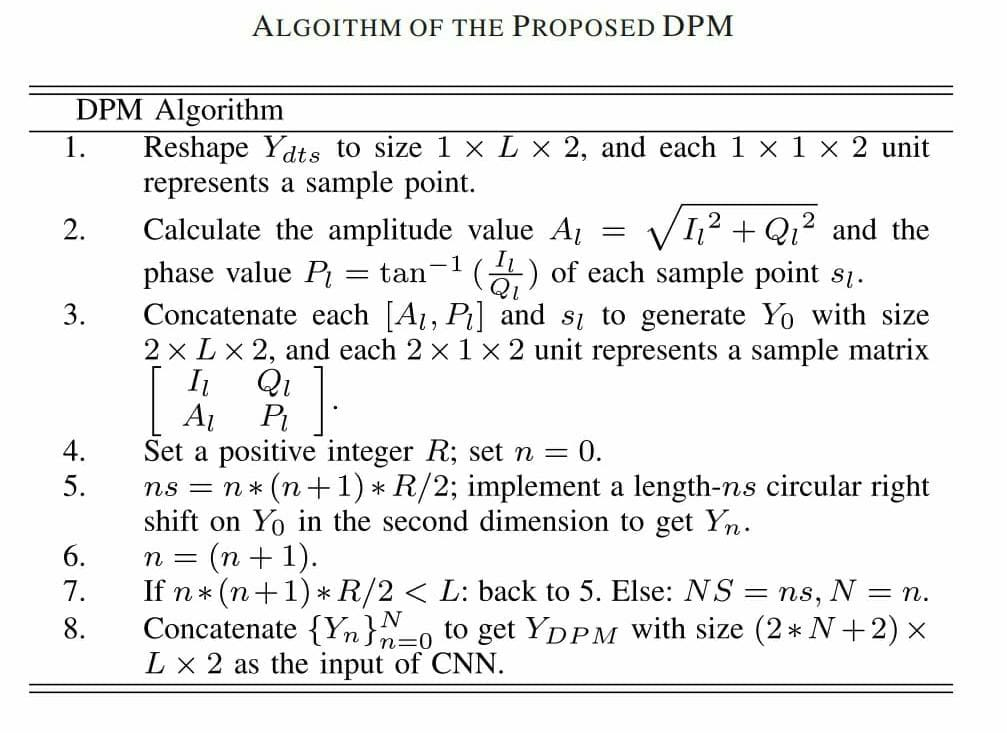
\includegraphics[width=0.9\textwidth]{algo.jpeg}
\end{figure}  
\end{frame}
\begin{frame}
      \begin{figure}[h]
    \centering
    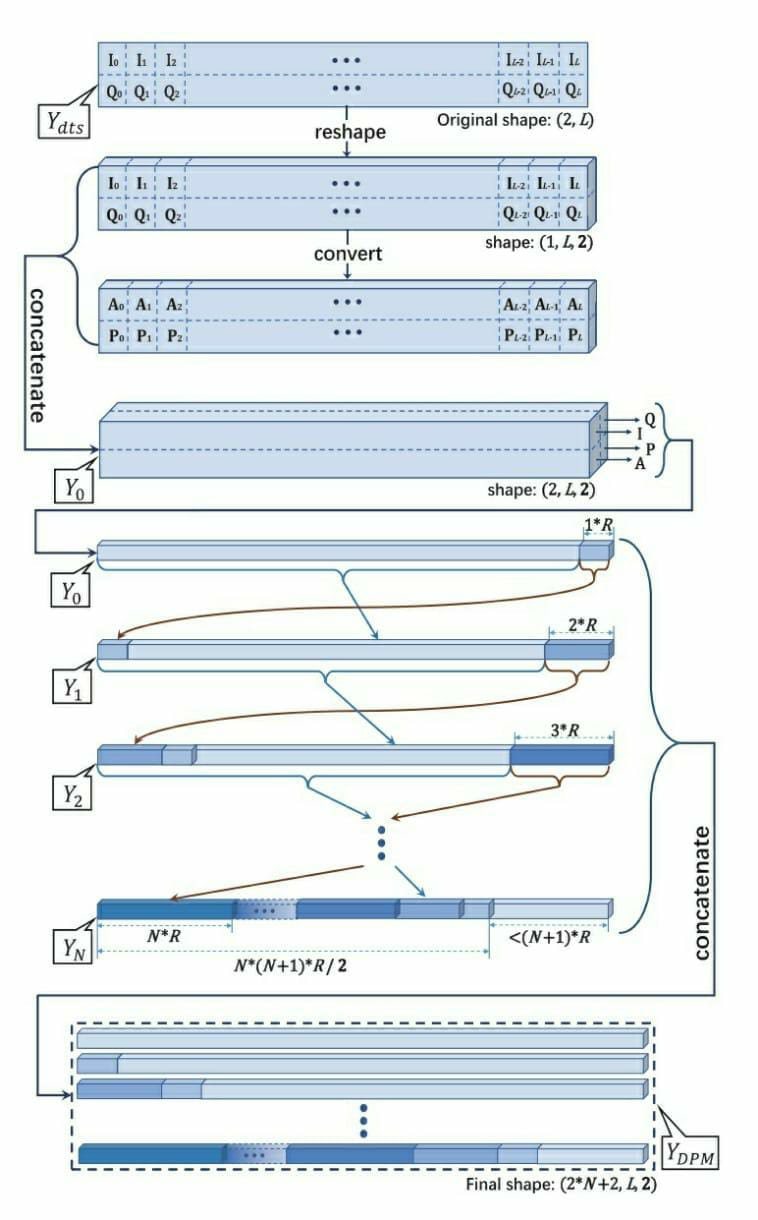
\includegraphics[width=0.45\textwidth]{descr.jpeg}
\end{figure}  
\end{frame}
\begin{frame}
\textbf{Structure of networks}\\
In this paper, we propose a specially designed CNN(SCNN) with residual blocks to identify the modulation scheme of DPM- processed signal dataset.
  \begin{figure}[h]
    \centering
    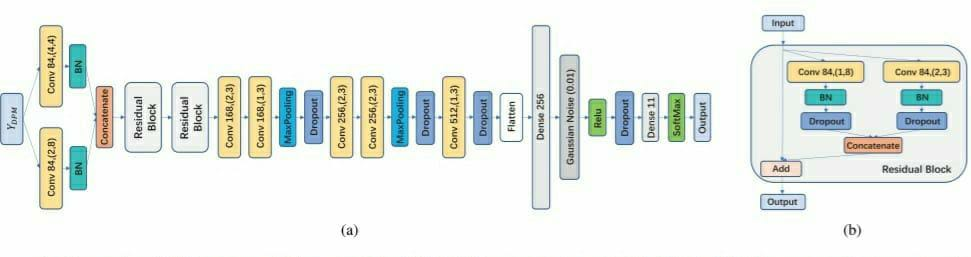
\includegraphics[width=\textwidth]{fig 2.jpeg}
\end{figure}  
\end{frame}
\begin{frame}
\begin{enumerate}[]
    \item The drop out rate of dropout layers is 0.5 and pool size of the pooling layer is 2$\times$ 2.
    \item All the convolutional layers use a rectified linear unit as the activation function.
    \item A gaussian noise layer is adopted to reduce the overfitting.
\end{enumerate}
 \begin{block}{The special designs in this network}
 \begin{enumerate}[]
     \item Each $2\times 1 \times 2$ unit in $\{Y_{n}\}_{n=0}^{N}$ is a sample point.
     \item The first two convolutional layers are parallel to each other. To focus on extracting the horizontal and vertical features, the fillers of these pairs of convolutional layers are set with a narrow shape and a comparably wide and short shape respectively. 
 \end{enumerate}
 \end{block}
\end{frame}
\begin{frame}{Experimental Results}
 \begin{figure}[h]
    \centering
    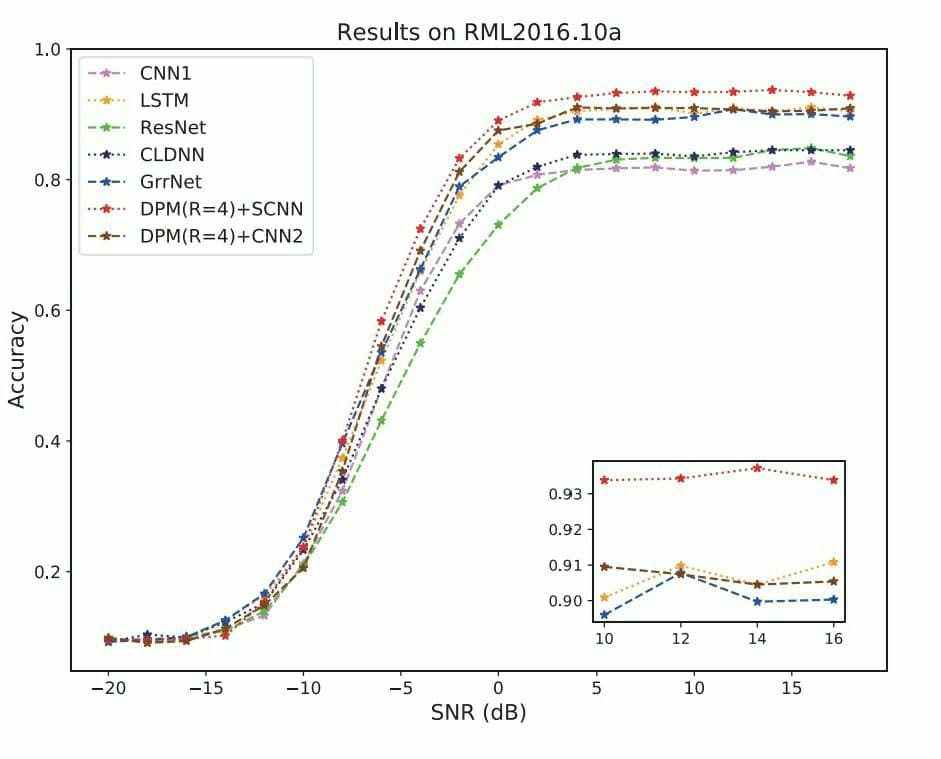
\includegraphics[width=0.7\textwidth]{fig 4.jpeg}
\end{figure} 
\end{frame}
\begin{frame}
     \begin{figure}[h]
    \centering
    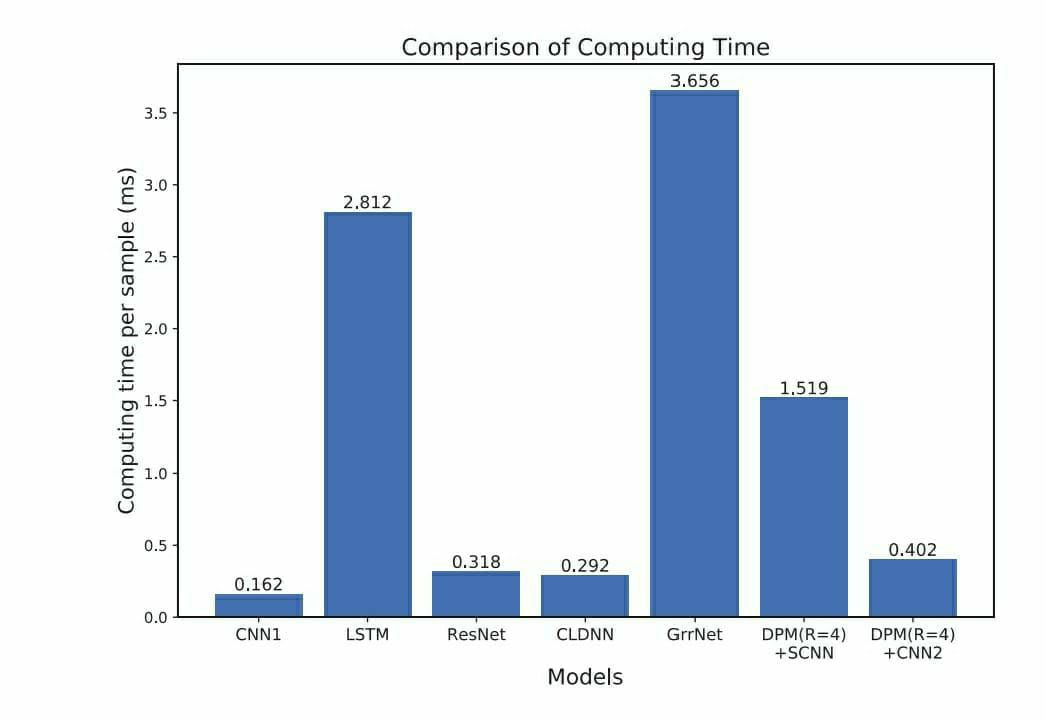
\includegraphics[width=0.7\textwidth]{fig 5.jpeg}
\end{figure} 
\end{frame}

\begin{frame}
     \begin{figure}[h]
    \centering
    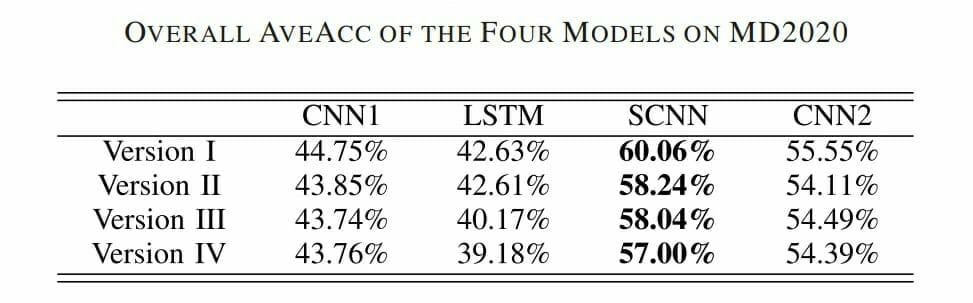
\includegraphics[width=\textwidth]{tab 3.jpeg}
\end{figure} 
\end{frame}
\end{document}